\chapter{Background}
For two blockchains to be interoperable, they must understand what happened in them, they must understand their data structure.
Since \cite{Nakamoto..09}, merkle trees are widely used in blockchain. We introduce merkle trees and inclusion proofs and how they are used in blockchain. You can also follow the notebook \cite{inclusionproofsnotebook} in order to better understand this chapter.
\section{Merkle tree \cite{merkle1988digital}}
Ralph Merkle invented the Merkle trees in 1979. We present here the binary Merkle tree used in Bitcoin. We present also a derivation of the Patricia trie used in ethereum in \ref{Merkle:ethereum}.
\subsection{Binary Merkle tree}
\begin{figure}[H]
    \centering
\includegraphics[width=0.7\linewidth]{background/Merkle.png}
    \caption{Binary Merkle tree from \cite{wikimerkle}}
    \label{fig:Merkle}
\end{figure}
A binary Merkle tree is the result of hashing  blockchain transaction two by two: 
\begin{enumerate}
    \item List all the data that need to be saved in an ordered list: it can be $n$ user ids, for example, or any kind of data. In blockchain, these data are the transactions. Here say we have 4 transactions L1, L2, L3, and L4.
    \item Hash these data one by one to obtain $n$ hashes. Here we obtain 4 transactions hashes \\($Hash_{0-0},Hash_{0-1},Hash_{1-0},Hash_{1-1})$
    \item Hash the hashes two by two starting from the left. If there is only one node on the right of the tree, we duplicate it to obtain the parent. Here we obtain $Hash_0$ and $Hash_1$.
    \item Repeat the last step until we obtain only one node left: the root.
\end{enumerate}
The root is a fingerprint of all the data, in our case the four transactions. 
It means that if one changes anything in the original data, the timestamp of the first transaction, for example, it'll change completely the root hash of the Merkle tree, thanks to the non-locality property of the hash function used (Alice and Aline have very different hashes even if they have only one different letter). The security of Merkle trees relies on the collision resistance of their hash function.  

To better understand this process, we'll take the example of a bitcoin Merkle tree for the block \href{https://blockchair.com/bitcoin/block/170861}{170 861}:

\begin{figure}[H]
    \centering
\begin{tikzpicture}
\tikzset{edge from parent/.style={draw,edge from parent path={(\tikzparentnode.south)-- +(0,-8pt)-| (\tikzchildnode)}}}
\Tree 
[.acb5aeb
[.e2d23ad
[.8e45845 [.338bbd0 ] [.1ad1138 ] ]
[.85b994b [.c77834d ] [.bb3d833 ] ] ]
[.13f0f97
[.e2c81be [.38d563c ] [.8fc0507 ] ]
[.9511f44 [.9db9fe6 ] [.3c72fdb ] ] ] ]
\end{tikzpicture}
    \caption{Merkle tree of the bitcoin block \href{"https://blockchair.com/bitcoin/block/170861"}{170 861}}
    \label{fig:Merkletree}
\end{figure}

\subsection{Proof of inclusion} \label{Merkle:inclusion}
\iffalse
  \begin{forest}
    for tree={
      edge={{Stealth[]}-},
    }
    [acb5aeb
      [e2d23ad
        [8e45845
          [338bbd0]
            [1ad1138]
            ]
            [85b994b
                [\colorbox{lime}{c77834d}]
                [bb3d833]
            ]
            ]
    [13f0f97
    [e2c81be
    [38d563c] [8fc0507]][9511f44 [9db9fe6][3c72fdb]]]
            ]
  \end{forest}
\fi

Merkle trees allow to summarize the data into one fixed-length fingerprint, the root hash. 
But why should we use this data structure instead of just hashing all the hashes for example?

This data structure allows proof of inclusion. In the case of bitcoin for example, the data is the transactions, and this structure allows other users to answer the folloxing question: \textit{Is this transaction really included in that block?}

So let's consider the Merkle tree below from our example:


\begin{figure}[H]
    \centering

\begin{tikzpicture}
\tikzset{edge from parent/.style={draw,edge from parent path={(\tikzparentnode.south)-- +(0,-8pt)-| (\tikzchildnode)}}}
\Tree 
[.acb5aeb
[.e2d23ad
[.\colorbox{lime}{8e45845} [.338bbd0 ] [.1ad1138 ] ]
[.85b994b [.\colorbox{yellow}{c77834d} ] [.\colorbox{lime}{bb3d833} ] ] ]
[.\colorbox{lime}{13f0f97}
[.e2c81be [.38d563c ] [.8fc0507 ] ]
[.9511f44 [.9db9fe6 ] [.3c72fdb ] ] ] ]
\end{tikzpicture}
    \caption{Proof of inclusion: Transaction to be verified in yellow, Merkle proof in green}
    \label{fig:Merkleproof}
\end{figure}


We have 8 transaction hashes that we want to place in the Merkle tree in this example. Let's say we are interested in the transaction in yellow (c77834d) because it's directer towards to our account. We want a proof that this transaction has really happened, and has been included in the block with Merkle root acb5aeb. 

The proof is a Merkle block with the green hashes. The verifier of this proof can then follow these steps.
\begin{enumerate}
    \item With the yellow transaction and the green one bb3d833 you can concatenate and hash it to get the parent hash 85b994b.
    \item With this last hash 85b994b and the green one 8e45845 you can concatenate and hash them to get the parent hash e2d23ad.
    \item And with this last hash concatened with the last green one 13f0f97 and hashed, we get the Merkle root
    \item We compare the calculated Merkle root from the proof and the real one from the block. If they match, the proof is accepted.
    In Bitcoin, it means that the transaction is included in this block. If it doesn't, we cannot prove the inclusion with that proof. 
\end{enumerate} 
\subsection{Proof scaling}
\textbf{
What is the advantage of using this data structure?}

The verifier only needs the Merkle root of the block to accept the proof of inclusion. But as this is a binary tree, the number of hashes at each level is divided by two, so this proof only consists of $\log_2(n)$ hashes, with $n$ the number of transactions. 
It means that if we have 8 transactions, as in this example we  need one hash per level so $\log_2(8)=3$ hashes to prove the inclusion of the transaction in the block.

\textit{
If $n=100$ we need $\log_2(100)\sim 7$ hashes; if $n=1000$ we need $\log_2(1000)\sim 10$ hashes.
}


Now there is a trade off. You can reduce the height of the tree by making it wider. Instead of two children and the binary tree from Bitcoin, we can have 16 children (plus the value) like in Ethereum. This has a drawback as it increases the length of the proof. 
\begin{figure}[H]
    \centering
    \includegraphics[width=0.7\linewidth]{background/Merklescaling.png}
    \caption{Merkle tree proof scaling \cite{merkleproofscaling}}
    \label{fig:Merklewidth}
\end{figure}

The general formula for calculating the proof's length is $\text{length}_{proof}=(m-1)\log_m(n)$ with $n$ leaves of width $m$.

Note that 
Verkle trees \cite{verkle} are an interesting solution to this problem.

\subsection{Some applications}
\textbf{Merkle trees play a key role in distributed systems} because the same data should exist in multiple places. Here the data integrity property is important.

\textbf{Blockchains}, since the appearance of their white paper, use the Merkle trees to represent data. This allows data integrity as for any distributed systems but also allows the light nodes to just download the fingerprint of the data.  

\textbf{Sismo}~\cite{sismo} manages groups of accounts represented in Merkle trees. Accounts are a key value pair: the key is the identifier, usually the address of the user, and the value depends on the group. The groups are for example Twitter accounts, where the value is the number of followers, or github contributors, where the value is the number of commits. 
\begin{figure}[H]
    \centering
    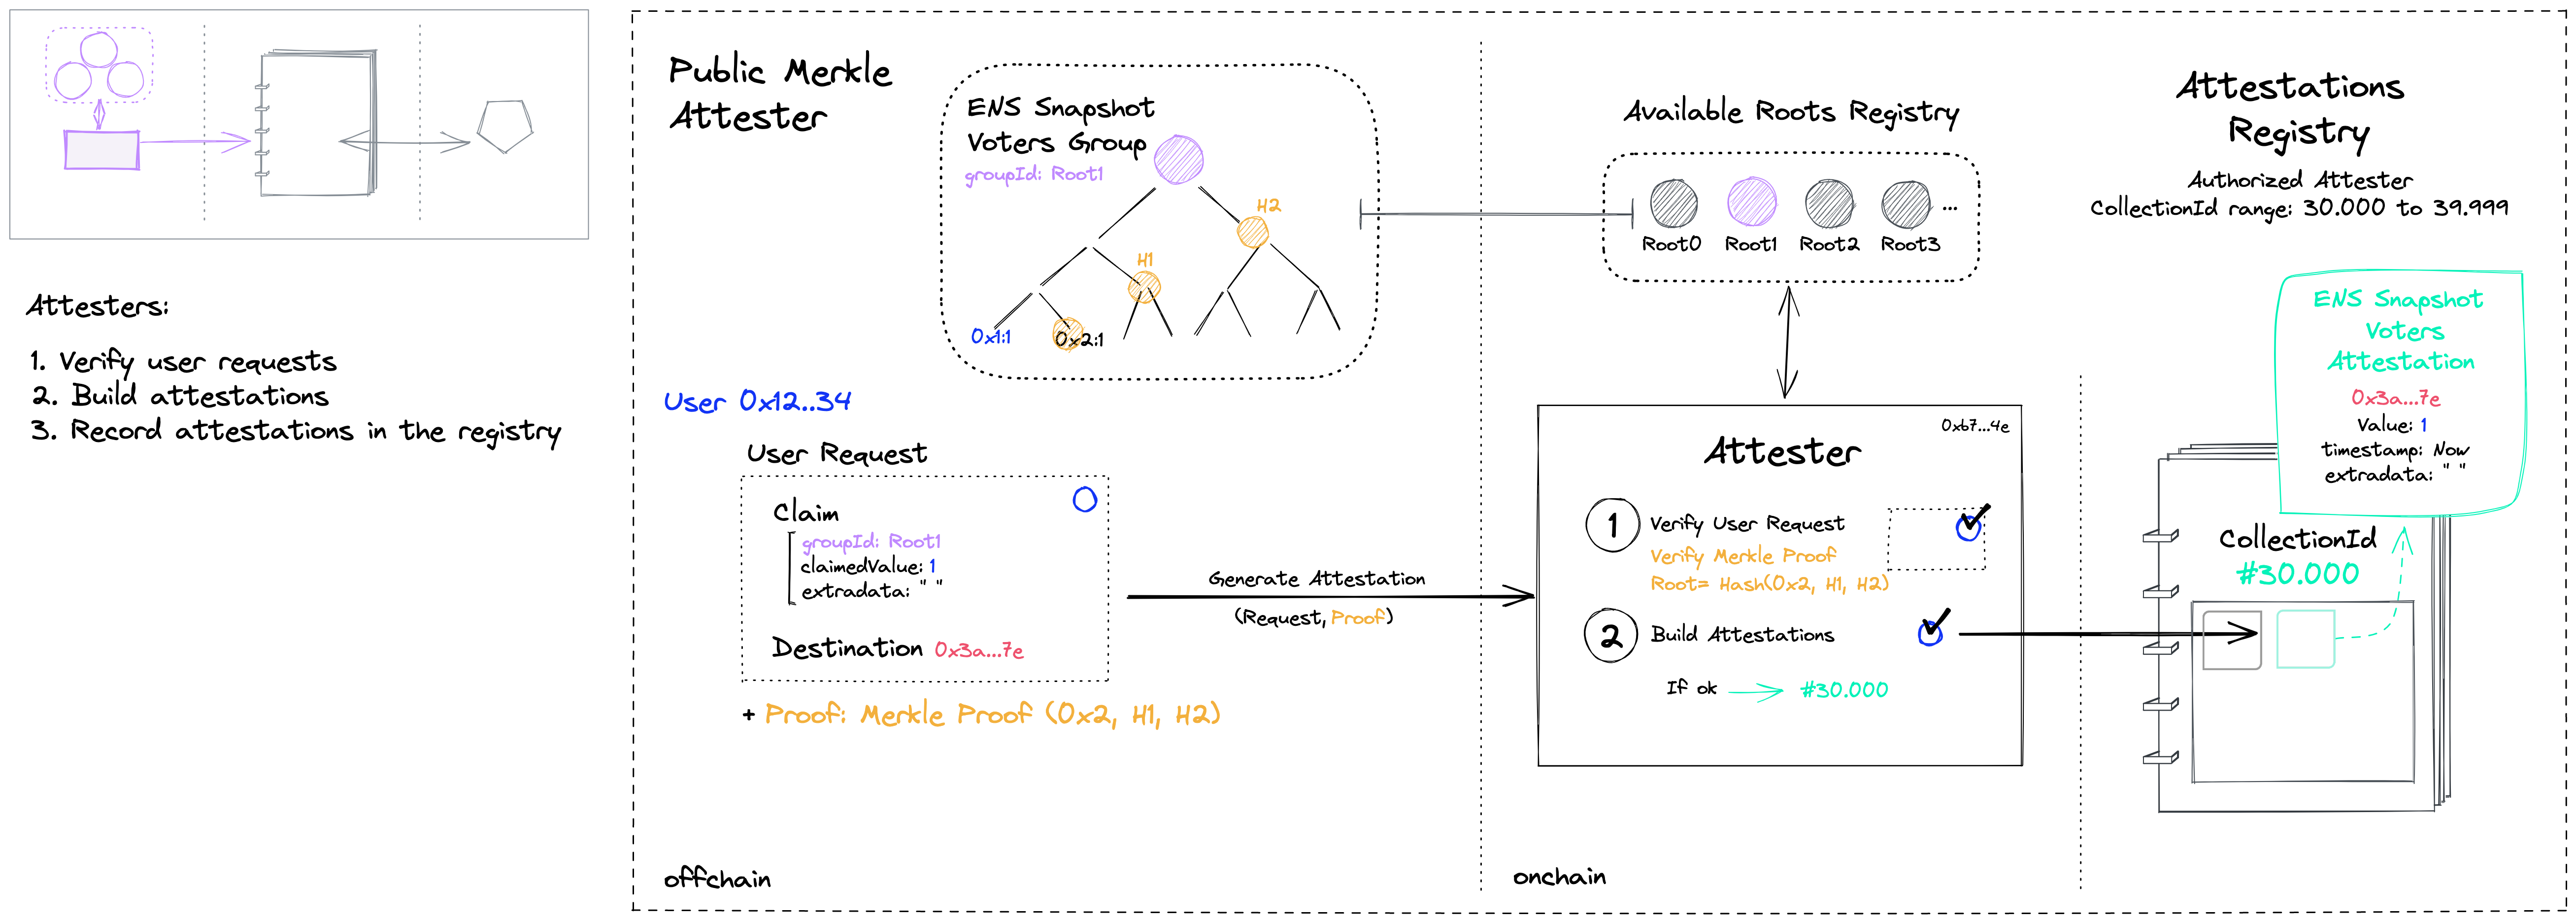
\includegraphics[width=1.\linewidth]{background/sismo2.png}
    \caption{Sismo: users claim their attestation.\cite{sismo}}
    \label{fig:sismo}
\end{figure}


\subsection{Ethereum tree}
Binary Merkle tree are used in Bitcoin. 
In Ethereum a more complicated version is used, derived from the Patricia trie. First let's understand what a trie is. 
\subsubsection{Trie}
\begin{figure}[H]
    \centering
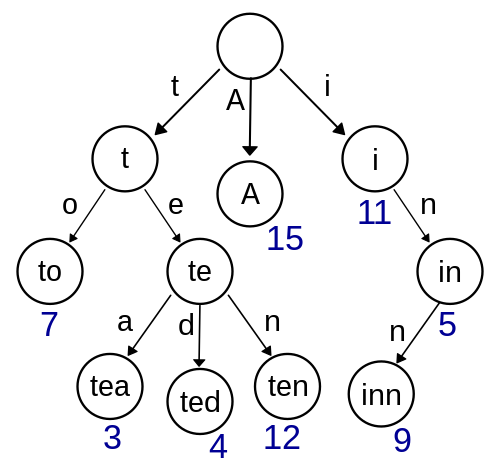
\includegraphics[width=0.3\linewidth]{background/trie.png}
    \caption{Trie representing the words "A", "to", "tea", "ted", "ten", "i", "in", and "inn"}
    \label{fig:trie}
\end{figure}
A trie is a tree data structure where the key of the node is also his path from the root. The key is usually a string.
In other words positions in the trie are determined directly from the key and the inverse is correct. 

Let's say you want to save $n$ words in the trie.
\begin{enumerate}
    \item From the root, at step 1 we take the first letter of each of the $n$ words and create a leaf for each different ones. In the example from the figure above, we  take A from A, t from to, tea, ted, ten, i from i, in and inn. We have then 3 nodes from the root: t, A, and i.
    \item At step $t$, repeat the first step but instead take the $t$ first letters. 
    \item Stop when all the original words are in a leaf. 
\end{enumerate}
If we have a string with 200 letters, we'll have to create 200 levels.
\subsection{Patricia trie}
As said in the last section, if you have a $n$-length word you'll have to create $n$ levels, which is not optimized in term of storage. 
Instead, radix trees and Patricia tries are a compressed version of the above trie.
\begin{figure}[H]
    \centering
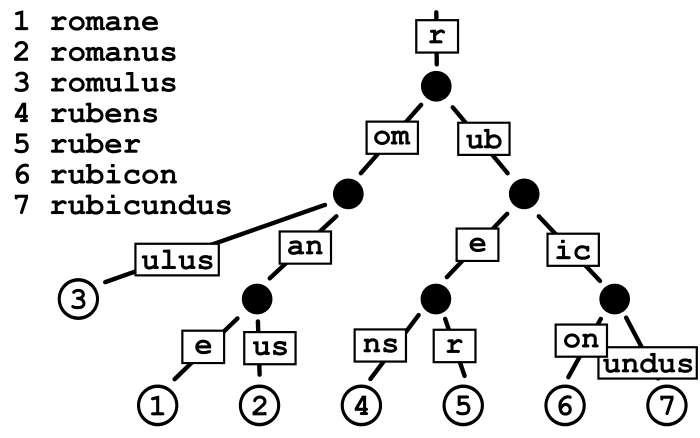
\includegraphics[width=0.4\linewidth]{background/patricia.png}
    \caption{Patricia trie}
    \label{fig:patricia}
\end{figure}
Here, we are not limited at each step in terms of length of the key.

\subsection{Patricia Merkle trie}
\label{Merkle:ethereum}
\begin{figure}[H]
    \centering
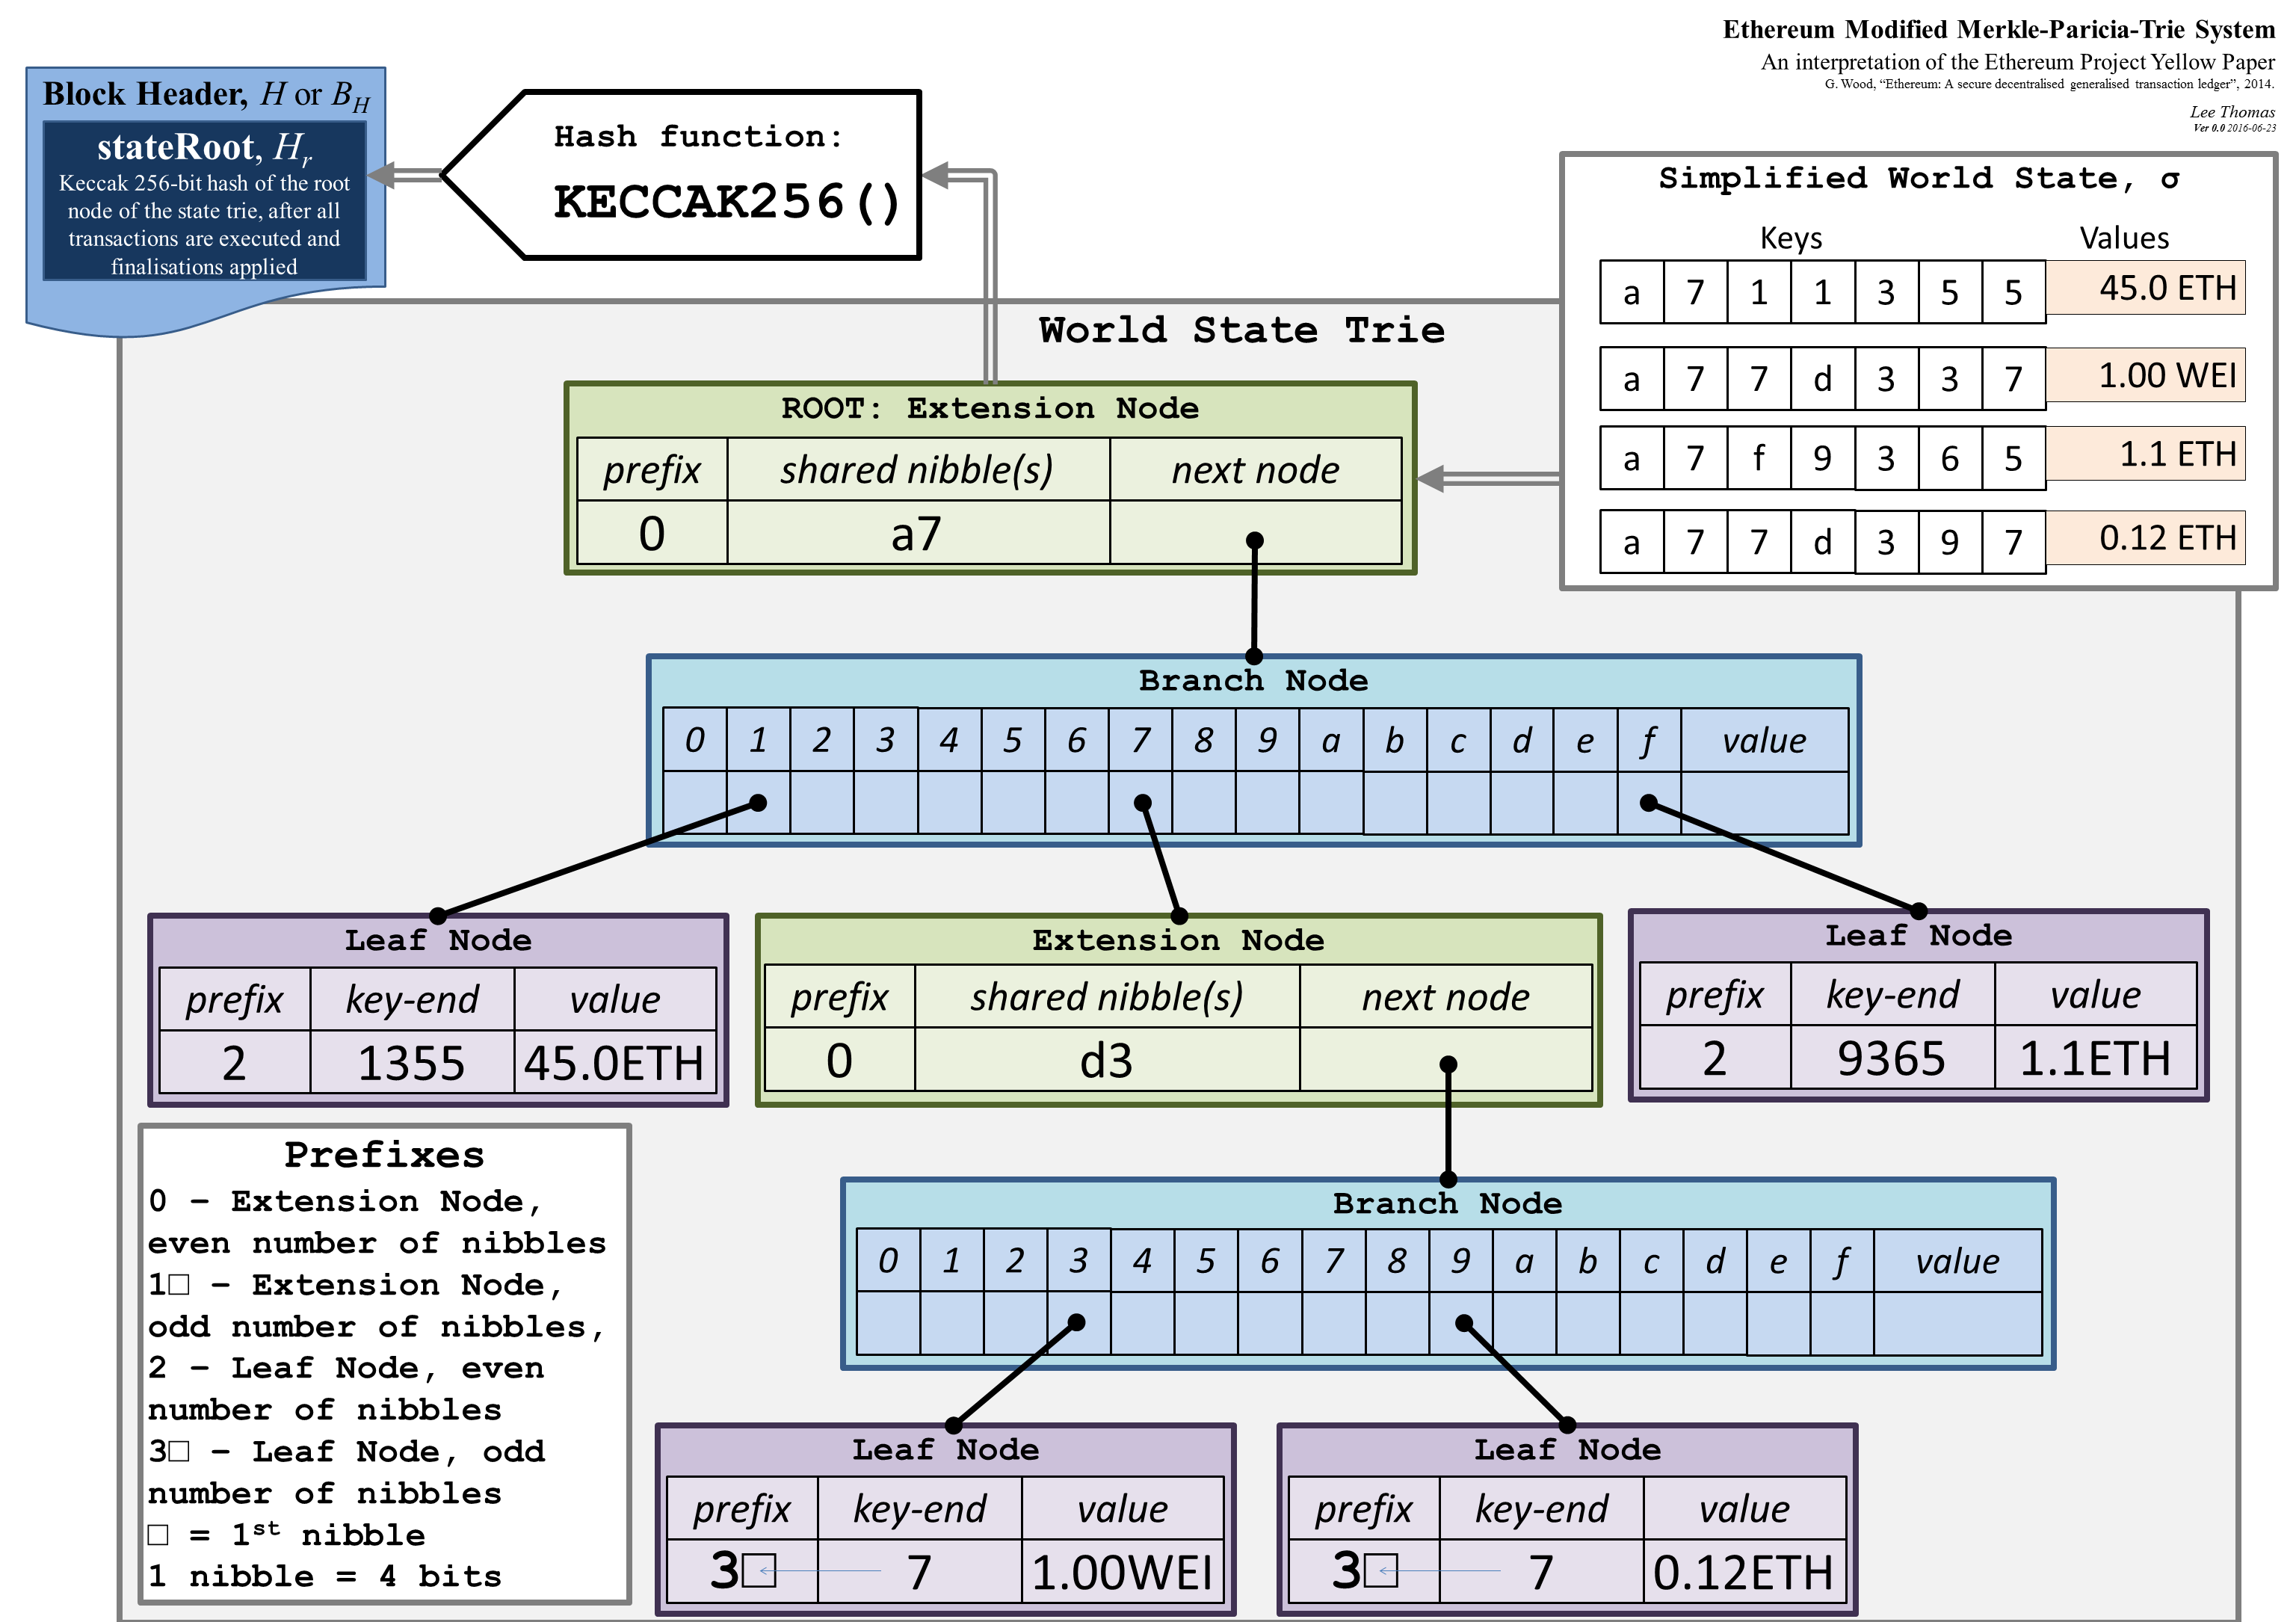
\includegraphics[width=0.9\linewidth]{background/ethereum_mpt.png}
    \caption{Ethereum Patricia trie}
    \label{fig:eth_mpt}
\end{figure}

The Patricia Merkle trie used in Ethereum modifies the original Patricia trie. The keys are hexadecimal strings and defines 4 types of nodes: 
\begin{itemize}
    \item EmptyNode, represented as the empty string;
    \item BranchNode, a 17-item node [v0 ... v15, vt];
    \item LeafNode, a 2-item node [encodedPath, value];
    \item ExtensionNode, a 2-item node [encodedPath, key].
\end{itemize}
A branch node at a certain step $t$, at letter t, is created when there are multiple possible letters for the next letter at $t+1$. Since we use hexadecimal keys, at each step we can choose between 16 letters (or the value).

A leaf node is the last possible node in the branch and contains the value. Here we can say that the key represents the address of an Ethereum account, and the value is the balance. 

The extension node is the compression offered by the Patricia trie. It represents the shared nibbles (letters) before two or more words diverge. 



Ethereum~\cite{Buterin..13} stores three Merkle roots in the block header: one for the transactions, as in Bitcoin, another one for the state (balances for example), and another one for the receipts. 


\section{Blockchain basics}

A blockchain can be viewed as a replicated state machine. It means that  each time $t$ is associated with a global state that goes to the next state at $t+1$ with the state transition function. 

Here the state is for example account balances for Bitcoin, and the state transition function represented by the transactions, instructions to be executed to go to the next state.
In blockchains, the transactions for each state transition are placed in a new block, adding to the chain of blocks.
\begin{figure}[H]
\centering
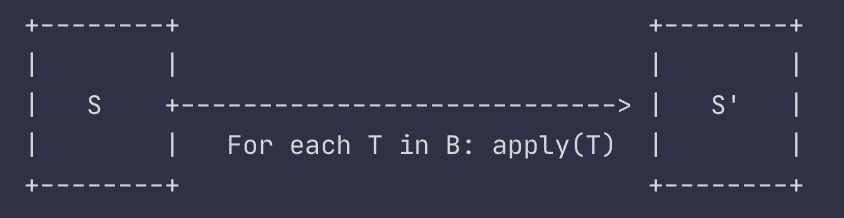
\includegraphics[width=0.6\linewidth]{background/state_transition.png}
    \caption{The state $S$ transitioning to state $S'$ by executing all transactions $T$ from the block $B$ \cite{statemachine}}
    \label{fig:state_transition}
\end{figure}
Lastly, it is replicated across all the full nodes to ensure global consistency of the distributed ledger, meaning that the nodes on the network should agree on the blockchain state thanks to the consensus algorithm.

\subsection{The block}
So what is stored exactly in a block? 

Let's say for the moment that a Bitcoin block consists of:
\begin{itemize}
    \item the hash of the previous block (you take the whole previous block and pass it to the hash function);
    \item the nonce resulting from the cryptographic puzzle (we'll talk about it later); 
    \item the list of transactions included in the block.
\end{itemize}
\begin{figure}[H]
    \centering
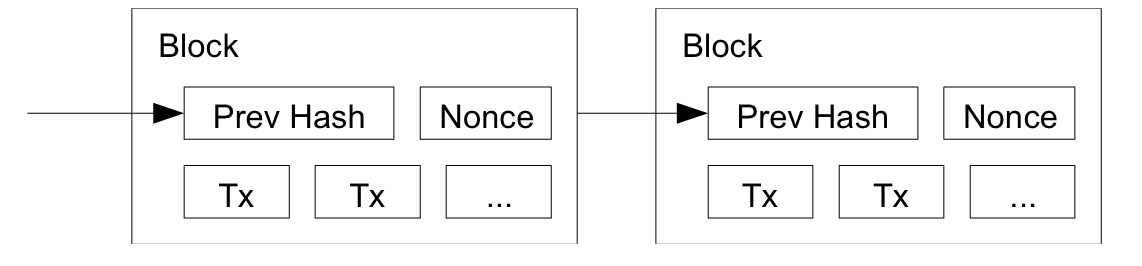
\includegraphics[width=0.6\linewidth]{background/block.png}
    \caption{A Bitcoin block: the hash of the previous block, the nonce, and the list of transactions \cite{Nakamoto..09}}
    \label{fig:block}
\end{figure}

This requires every node in the network to keep the list of transactions since 2009.

\subsection{Merkle tree of transactions}
In fact, the block is composed of the block header and the list of transactions. The block header contains this time the root hash of the transactions Merkle tree.
The root hash is a summary of all the transactions happening during that period represented a Merkle tree. For Bitcoin, binary Merkle tree are used for transactions, whereas, in Ethereum, Merkle Patricia trees are used to store transactions, state, and receipts. 
\begin{figure}[H]
    \centering
\includegraphics[width=0.4\linewidth]{background/blockMerkle.png}
    \caption{A Bitcoin~\cite{Nakamoto..09} block}
    \label{fig:blockMerkle}
\end{figure}

\subsection{Single payment verification}

In~\cite{Nakamoto..09}, the author mentioned merkle inclusion proofs to verify payment, but in order to keep only the block headers in the blockchain. For security reasons this never happened. 

Instead this technique allowed two actors to emerge.

A \textbf{full node} stores all the full blocks, with the transactions. With these transactions, it can provide the proof of inclusion: the hashes required to prove a transaction is in a particular block.

A \textbf{light node} asks for the blocks headers to the full nodes of the network. Once it got the block headers, it can ask the full nodes of the network to provide a proof for the transactions it is interested in. With the procedure described in Section~\ref{Merkle:inclusion}, the light node can verify that a specific transaction has indeed happened in the blockchain.

A light node is only storing the block headers, so even a phone can handle the amount of storage needed. This allows for example to verify with your wallet that a transaction has been executed  on your laptop without downloading the $\sim 500$GB of the blockchain.


\subsection{Security of light clients}
\label{background:security}
We now share some security considerations about the block headers validity/finality. The light clients are able to verify the proofs of inclusion against the block header Merkle root. But how can they trust this block header? Is it final ? Is it valid? 

\subsubsection{Proof of work}
In Bitcoin, with the proof-of-work mechanism, light clients ask the full nodes for the last block headers and select the longest chain. 
A block in Bitcoin and with proof of work contains a nonce (number generated once). This nonce represents the amount of work done by the validator to submit this block. 
Indeed the miners, full nodes with the ability to produce blocks, try to solve a cryptographic puzzle. This puzzle consists in testing all values of the nonce until they find one that makes the hash of the block (including the nonce) starting with a certain number of zeros. 
In other words, they have to brute-force search a nonce such that the block hash meets the required level of difficulty: the number of zeros. 
For example, if we ask the miners to find a hash of the block with only one zero, it'll be pretty easy. If we ask them to find a block hash with 10 starting zero, it'll be a lot more difficult. 

This nonce is the probabilistic guarantee that the block header is valid. The more blocks accepted (with a nonce then) after that block confirm that the transactions for this block and block header are valid and will not be reverted.

\subsubsection{Proof of stake}
\label{securitylc:pos}
If the proof-of-work mechanism relies on the amount of work done to ensure the security of the light client, the security of the proof-of-stake light client is a less obvious. 

As a proof-of-stake light client, we can get the genesis header and sync to the latest block header from it. But it's slow and unsafe because it's costless for a hacker to fork the network at some point and produce invalid blocks (long-range attacks). 
Instead, a light client can ask a trusted source for header that is not in the unbounding window. It means that the trusted source, full node, can be slashed if it gives the light client fake block headers. The trusted source can be someone you know, a friend or a verified website for example.

We recall that the Ethereum 2.0 has a sync committee of 512 validators randomly chosen every 27 hours; it is responsible for signing every block header during that period. If at least 2/3 of the validators sign a given block header, the block is considered finalized and the network state is valid. 
This last consideration is important for the solutions presented in the next chapter.



\section{Zero knowledge}
\label{zeroknowledge}
This section is meant to be a light introduction to the zero-knowledge-proof concept to understand interoperability solutions. 

A zero-knowledge protocol is a method by which one party (the prover) can prove to another party (the verifier) that something is true, without revealing any information apart from the fact that this specific statement is true~\cite{Goldwasser}.

For example, in the case of digital signatures, you send a signature proving that you are indeed the one sending the mail. More precisely, this signature proves that you know the private key without revealing it. The verifier checks that the signature matches the public key of the sender ($\sim$ the signature reveals the public key)

Instead of only proving that you know the private key as in digital signatures, zero-knowledge proofs can prove "any type" of computation. For example, you can prove that: 
\begin{itemize}
    \item you know $m$ such that $SHA_3(m)=0$ to the verifier, without revealing $m$; 
    \item you know a sudoku solution to a sudoku problem without revealing it;
    \item you know the $1000^{th}$ Fibonacci number (defined by the suite $a_{n-2}+a_{n-1}=a_n$);
    \item some transactions are valid, thus allowing for instance ZK roll-ups to process transactions off chain, and prove on-chain to Layer 1 that these transactions are indeed valid. 
\end{itemize}

In fact, zero-knowledge (ZK) proofs can offer computational integrity and privacy (with zero knowledge). Privacy is not always necessary and ZK can be used only for the computational integrity property. 
\begin{description}
    \item[Computational integrity] proves that you have done the right computation, even when no one is watching. For example, in ZK rollups,  computational integrity is the main need, and the privacy is not always/often taken into account.
    \item[Privacy] with zero knowledge ensures thaty you don't reveal anything about the statement. In Zerocash~\cite{sasson2014zerocash}, privacy is needed to ensure the confidentiality of the transactions.
\end{description}

A zero-knowledge protocol should verify the following properties.
\begin{description}
    \item[Completeness] If the claim is valid, the verifier accepts the proof.
\item[Soundness] If the claim is invalid, the verifier should reject the proof with very high probability.

\item[Zero-knowledge] The verifier learns nothing about a statement beyond its validity or falsity.
\end{description}

To conclude, some important properties are expected from these protocols. We want  short proofs in terms of size, for example. We also want, and this is a fundamental requirement, very fast verifications. If the prover with a highly efficient computer computes the hash of a 200GB document, the verification should be very fast and consists in a much lighter computation than the prover's one.

This last requirement is at the heart of the zero-knowledge research and explains the complexity of the techniques used.
